% Created by tikzDevice version 0.12.3 on 2019-12-11 20:53:30
% !TEX encoding = UTF-8 Unicode
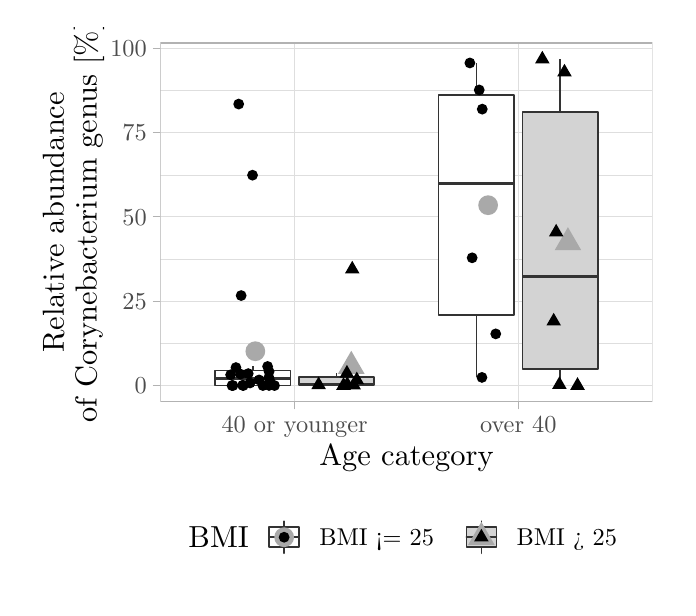
\begin{tikzpicture}[x=1pt,y=1pt]
\definecolor{fillColor}{RGB}{255,255,255}
\path[use as bounding box,fill=fillColor,fill opacity=0.00] (0,0) rectangle (231.26,202.36);
\begin{scope}
\path[clip] (  0.00,  0.00) rectangle (231.26,202.36);
\definecolor{drawColor}{RGB}{255,255,255}
\definecolor{fillColor}{RGB}{255,255,255}

\path[draw=drawColor,line width= 0.6pt,line join=round,line cap=round,fill=fillColor] (  0.00,  0.00) rectangle (231.26,202.36);
\end{scope}
\begin{scope}
\path[clip] ( 47.99, 67.14) rectangle (225.76,196.86);
\definecolor{fillColor}{RGB}{255,255,255}

\path[fill=fillColor] ( 47.99, 67.14) rectangle (225.76,196.86);
\definecolor{drawColor}{gray}{0.87}

\path[draw=drawColor,line width= 0.1pt,line join=round] ( 47.99, 88.28) --
	(225.76, 88.28);

\path[draw=drawColor,line width= 0.1pt,line join=round] ( 47.99,118.75) --
	(225.76,118.75);

\path[draw=drawColor,line width= 0.1pt,line join=round] ( 47.99,149.23) --
	(225.76,149.23);

\path[draw=drawColor,line width= 0.1pt,line join=round] ( 47.99,179.71) --
	(225.76,179.71);

\path[draw=drawColor,line width= 0.3pt,line join=round] ( 47.99, 73.04) --
	(225.76, 73.04);

\path[draw=drawColor,line width= 0.3pt,line join=round] ( 47.99,103.52) --
	(225.76,103.52);

\path[draw=drawColor,line width= 0.3pt,line join=round] ( 47.99,133.99) --
	(225.76,133.99);

\path[draw=drawColor,line width= 0.3pt,line join=round] ( 47.99,164.47) --
	(225.76,164.47);

\path[draw=drawColor,line width= 0.3pt,line join=round] ( 47.99,194.95) --
	(225.76,194.95);

\path[draw=drawColor,line width= 0.3pt,line join=round] ( 96.47, 67.14) --
	( 96.47,196.86);

\path[draw=drawColor,line width= 0.3pt,line join=round] (177.28, 67.14) --
	(177.28,196.86);

\path[] ( 81.32,105.56) circle (  1.96);

\path[] ( 81.32,149.06) circle (  1.96);

\path[] ( 81.32,174.75) circle (  1.96);
\definecolor{drawColor}{gray}{0.20}

\path[draw=drawColor,line width= 0.6pt,line join=round] ( 81.32, 78.46) -- ( 81.32, 79.94);

\path[draw=drawColor,line width= 0.6pt,line join=round] ( 81.32, 73.06) -- ( 81.32, 73.04);

\path[draw=drawColor,line width= 0.6pt,line join=round,line cap=round,fill=fillColor] ( 67.69, 78.46) --
	( 67.69, 73.06) --
	( 94.96, 73.06) --
	( 94.96, 78.46) --
	( 67.69, 78.46) --
	cycle;

\path[draw=drawColor,line width= 1.1pt,line join=round] ( 67.69, 75.51) -- ( 94.96, 75.51);

\path[] (111.63,115.07) circle (  1.96);

\path[draw=drawColor,line width= 0.6pt,line join=round] (111.63, 76.24) -- (111.63, 77.44);

\path[draw=drawColor,line width= 0.6pt,line join=round] (111.63, 73.21) -- (111.63, 73.04);
\definecolor{fillColor}{RGB}{211,211,211}

\path[draw=drawColor,line width= 0.6pt,line join=round,line cap=round,fill=fillColor] ( 97.99, 76.24) --
	( 97.99, 73.21) --
	(125.26, 73.21) --
	(125.26, 76.24) --
	( 97.99, 76.24) --
	cycle;

\path[draw=drawColor,line width= 1.1pt,line join=round] ( 97.99, 73.37) -- (125.26, 73.37);

\path[draw=drawColor,line width= 0.6pt,line join=round] (162.13,178.12) -- (162.13,189.60);

\path[draw=drawColor,line width= 0.6pt,line join=round] (162.13, 98.59) -- (162.13, 75.98);
\definecolor{fillColor}{RGB}{255,255,255}

\path[draw=drawColor,line width= 0.6pt,line join=round,line cap=round,fill=fillColor] (148.49,178.12) --
	(148.49, 98.59) --
	(175.77, 98.59) --
	(175.77,178.12) --
	(148.49,178.12) --
	cycle;

\path[draw=drawColor,line width= 1.1pt,line join=round] (148.49,146.06) -- (175.77,146.06);

\path[draw=drawColor,line width= 0.6pt,line join=round] (192.43,171.80) -- (192.43,190.96);

\path[draw=drawColor,line width= 0.6pt,line join=round] (192.43, 79.08) -- (192.43, 73.04);
\definecolor{fillColor}{RGB}{211,211,211}

\path[draw=drawColor,line width= 0.6pt,line join=round,line cap=round,fill=fillColor] (178.80,171.80) --
	(178.80, 79.08) --
	(206.07, 79.08) --
	(206.07,171.80) --
	(178.80,171.80) --
	cycle;

\path[draw=drawColor,line width= 1.1pt,line join=round] (178.80,112.35) -- (206.07,112.35);
\definecolor{fillColor}{RGB}{169,169,169}

\path[fill=fillColor] (116.93, 85.60) --
	(121.73, 77.28) --
	(112.12, 77.28) --
	cycle;

\path[fill=fillColor] ( 82.27, 85.45) circle (  3.57);

\path[fill=fillColor] (195.22,130.27) --
	(200.03,121.94) --
	(190.42,121.94) --
	cycle;

\path[fill=fillColor] (166.38,138.21) circle (  3.57);
\definecolor{fillColor}{RGB}{0,0,0}

\path[fill=fillColor] (117.28,118.12) --
	(119.92,113.54) --
	(114.64,113.54) --
	cycle;

\path[fill=fillColor] (118.93, 78.09) --
	(121.57, 73.52) --
	(116.29, 73.52) --
	cycle;

\path[fill=fillColor] (115.36, 80.49) --
	(118.00, 75.92) --
	(112.71, 75.92) --
	cycle;

\path[fill=fillColor] (117.79, 76.21) --
	(120.43, 71.63) --
	(115.14, 71.63) --
	cycle;

\path[fill=fillColor] (105.13, 76.31) --
	(107.78, 71.74) --
	(102.49, 71.74) --
	cycle;

\path[fill=fillColor] (114.13, 76.09) --
	(116.77, 71.51) --
	(111.48, 71.51) --
	cycle;

\path[fill=fillColor] (115.49, 76.42) --
	(118.14, 71.85) --
	(112.85, 71.85) --
	cycle;

\path[fill=fillColor] ( 87.16, 75.94) circle (  1.96);

\path[fill=fillColor] ( 89.19, 73.04) circle (  1.96);

\path[fill=fillColor] ( 75.26, 79.54) circle (  1.96);

\path[fill=fillColor] ( 74.17, 73.04) circle (  1.96);

\path[fill=fillColor] ( 73.84, 73.04) circle (  1.96);

\path[fill=fillColor] ( 80.33, 73.96) circle (  1.96);

\path[fill=fillColor] ( 77.14,105.56) circle (  1.96);

\path[fill=fillColor] ( 83.63, 75.07) circle (  1.96);

\path[fill=fillColor] ( 77.69, 73.15) circle (  1.96);

\path[fill=fillColor] ( 87.23, 78.10) circle (  1.96);

\path[fill=fillColor] ( 86.70, 79.94) circle (  1.96);

\path[fill=fillColor] ( 87.23, 73.07) circle (  1.96);

\path[fill=fillColor] ( 85.01, 73.04) circle (  1.96);

\path[fill=fillColor] ( 81.25,149.06) circle (  1.96);

\path[fill=fillColor] ( 76.25,174.75) circle (  1.96);

\path[fill=fillColor] ( 76.92, 77.17) circle (  1.96);

\path[fill=fillColor] ( 73.34, 76.92) circle (  1.96);

\path[fill=fillColor] ( 77.90, 73.04) circle (  1.96);

\path[fill=fillColor] ( 87.70, 74.29) circle (  1.96);

\path[fill=fillColor] ( 79.69, 77.35) circle (  1.96);

\path[fill=fillColor] (198.69, 76.09) --
	(201.33, 71.51) --
	(196.04, 71.51) --
	cycle;

\path[fill=fillColor] (193.97,189.31) --
	(196.61,184.73) --
	(191.33,184.73) --
	cycle;

\path[fill=fillColor] (190.07, 99.33) --
	(192.72, 94.75) --
	(187.43, 94.75) --
	cycle;

\path[fill=fillColor] (190.97,131.48) --
	(193.61,126.90) --
	(188.33,126.90) --
	cycle;

\path[fill=fillColor] (192.14, 76.40) --
	(194.78, 71.82) --
	(189.50, 71.82) --
	cycle;

\path[fill=fillColor] (185.97,194.01) --
	(188.61,189.43) --
	(183.33,189.43) --
	cycle;

\path[fill=fillColor] (159.79,189.60) circle (  1.96);

\path[fill=fillColor] (164.26,172.92) circle (  1.96);

\path[fill=fillColor] (160.61,119.20) circle (  1.96);

\path[fill=fillColor] (164.15, 75.98) circle (  1.96);

\path[fill=fillColor] (169.14, 91.71) circle (  1.96);

\path[fill=fillColor] (163.17,179.85) circle (  1.96);
\definecolor{drawColor}{gray}{0.70}

\path[draw=drawColor,line width= 0.6pt,line join=round,line cap=round] ( 47.99, 67.14) rectangle (225.76,196.86);
\end{scope}
\begin{scope}
\path[clip] (  0.00,  0.00) rectangle (231.26,202.36);
\definecolor{drawColor}{gray}{0.30}

\node[text=drawColor,anchor=base east,inner sep=0pt, outer sep=0pt, scale=  0.88] at ( 43.04, 70.01) {0};

\node[text=drawColor,anchor=base east,inner sep=0pt, outer sep=0pt, scale=  0.88] at ( 43.04,100.48) {25};

\node[text=drawColor,anchor=base east,inner sep=0pt, outer sep=0pt, scale=  0.88] at ( 43.04,130.96) {50};

\node[text=drawColor,anchor=base east,inner sep=0pt, outer sep=0pt, scale=  0.88] at ( 43.04,161.44) {75};

\node[text=drawColor,anchor=base east,inner sep=0pt, outer sep=0pt, scale=  0.88] at ( 43.04,191.92) {100};
\end{scope}
\begin{scope}
\path[clip] (  0.00,  0.00) rectangle (231.26,202.36);
\definecolor{drawColor}{gray}{0.70}

\path[draw=drawColor,line width= 0.3pt,line join=round] ( 45.24, 73.04) --
	( 47.99, 73.04);

\path[draw=drawColor,line width= 0.3pt,line join=round] ( 45.24,103.52) --
	( 47.99,103.52);

\path[draw=drawColor,line width= 0.3pt,line join=round] ( 45.24,133.99) --
	( 47.99,133.99);

\path[draw=drawColor,line width= 0.3pt,line join=round] ( 45.24,164.47) --
	( 47.99,164.47);

\path[draw=drawColor,line width= 0.3pt,line join=round] ( 45.24,194.95) --
	( 47.99,194.95);
\end{scope}
\begin{scope}
\path[clip] (  0.00,  0.00) rectangle (231.26,202.36);
\definecolor{drawColor}{gray}{0.70}

\path[draw=drawColor,line width= 0.3pt,line join=round] ( 96.47, 64.39) --
	( 96.47, 67.14);

\path[draw=drawColor,line width= 0.3pt,line join=round] (177.28, 64.39) --
	(177.28, 67.14);
\end{scope}
\begin{scope}
\path[clip] (  0.00,  0.00) rectangle (231.26,202.36);
\definecolor{drawColor}{gray}{0.30}

\node[text=drawColor,anchor=base,inner sep=0pt, outer sep=0pt, scale=  0.88] at ( 96.47, 56.13) {40 or younger};

\node[text=drawColor,anchor=base,inner sep=0pt, outer sep=0pt, scale=  0.88] at (177.28, 56.13) {over 40};
\end{scope}
\begin{scope}
\path[clip] (  0.00,  0.00) rectangle (231.26,202.36);
\definecolor{drawColor}{RGB}{0,0,0}

\node[text=drawColor,anchor=base,inner sep=0pt, outer sep=0pt, scale=  1.10] at (136.88, 44.09) {Age category};
\end{scope}
\begin{scope}
\path[clip] (  0.00,  0.00) rectangle (231.26,202.36);
\definecolor{drawColor}{RGB}{0,0,0}

\node[text=drawColor,rotate= 90.00,anchor=base,inner sep=0pt, outer sep=0pt, scale=  1.10] at ( 13.08,132.00) {Relative abundance };

\node[text=drawColor,rotate= 90.00,anchor=base,inner sep=0pt, outer sep=0pt, scale=  1.10] at ( 24.96,132.00) { of Corynebacterium genus [\%]};
\end{scope}
\begin{scope}
\path[clip] (  0.00,  0.00) rectangle (231.26,202.36);
\definecolor{fillColor}{RGB}{255,255,255}

\path[fill=fillColor] ( 52.60,  5.50) rectangle (221.15, 30.95);
\end{scope}
\begin{scope}
\path[clip] (  0.00,  0.00) rectangle (231.26,202.36);
\definecolor{drawColor}{RGB}{0,0,0}

\node[text=drawColor,anchor=base west,inner sep=0pt, outer sep=0pt, scale=  1.10] at ( 58.10, 14.44) {BMI};
\end{scope}
\begin{scope}
\path[clip] (  0.00,  0.00) rectangle (231.26,202.36);
\definecolor{fillColor}{RGB}{255,255,255}

\path[fill=fillColor] ( 85.44, 11.00) rectangle ( 99.90, 25.45);
\end{scope}
\begin{scope}
\path[clip] (  0.00,  0.00) rectangle (231.26,202.36);
\definecolor{drawColor}{gray}{0.20}

\path[draw=drawColor,line width= 0.6pt,line join=round,line cap=round] ( 92.67, 12.45) --
	( 92.67, 14.61);

\path[draw=drawColor,line width= 0.6pt,line join=round,line cap=round] ( 92.67, 21.84) --
	( 92.67, 24.01);
\definecolor{fillColor}{RGB}{255,255,255}

\path[draw=drawColor,line width= 0.6pt,line join=round,line cap=round,fill=fillColor] ( 87.25, 14.61) rectangle ( 98.09, 21.84);

\path[draw=drawColor,line width= 0.6pt,line join=round,line cap=round] ( 87.25, 18.23) --
	( 98.09, 18.23);
\end{scope}
\begin{scope}
\path[clip] (  0.00,  0.00) rectangle (231.26,202.36);
\definecolor{fillColor}{RGB}{169,169,169}

\path[fill=fillColor] ( 92.67, 18.23) circle (  3.57);
\end{scope}
\begin{scope}
\path[clip] (  0.00,  0.00) rectangle (231.26,202.36);
\definecolor{fillColor}{RGB}{0,0,0}

\path[fill=fillColor] ( 92.67, 18.23) circle (  1.96);
\end{scope}
\begin{scope}
\path[clip] (  0.00,  0.00) rectangle (231.26,202.36);
\definecolor{fillColor}{RGB}{255,255,255}

\path[fill=fillColor] (156.72, 11.00) rectangle (171.17, 25.45);
\end{scope}
\begin{scope}
\path[clip] (  0.00,  0.00) rectangle (231.26,202.36);
\definecolor{drawColor}{gray}{0.20}

\path[draw=drawColor,line width= 0.6pt,line join=round,line cap=round] (163.95, 12.45) --
	(163.95, 14.61);

\path[draw=drawColor,line width= 0.6pt,line join=round,line cap=round] (163.95, 21.84) --
	(163.95, 24.01);
\definecolor{fillColor}{RGB}{211,211,211}

\path[draw=drawColor,line width= 0.6pt,line join=round,line cap=round,fill=fillColor] (158.53, 14.61) rectangle (169.37, 21.84);

\path[draw=drawColor,line width= 0.6pt,line join=round,line cap=round] (158.53, 18.23) --
	(169.37, 18.23);
\end{scope}
\begin{scope}
\path[clip] (  0.00,  0.00) rectangle (231.26,202.36);
\definecolor{fillColor}{RGB}{169,169,169}

\path[fill=fillColor] (163.95, 23.78) --
	(168.75, 15.45) --
	(159.14, 15.45) --
	cycle;
\end{scope}
\begin{scope}
\path[clip] (  0.00,  0.00) rectangle (231.26,202.36);
\definecolor{fillColor}{RGB}{0,0,0}

\path[fill=fillColor] (163.95, 21.28) --
	(166.59, 16.70) --
	(161.30, 16.70) --
	cycle;
\end{scope}
\begin{scope}
\path[clip] (  0.00,  0.00) rectangle (231.26,202.36);
\definecolor{drawColor}{RGB}{0,0,0}

\node[text=drawColor,anchor=base west,inner sep=0pt, outer sep=0pt, scale=  0.88] at (105.40, 15.20) {BMI <= 25};
\end{scope}
\begin{scope}
\path[clip] (  0.00,  0.00) rectangle (231.26,202.36);
\definecolor{drawColor}{RGB}{0,0,0}

\node[text=drawColor,anchor=base west,inner sep=0pt, outer sep=0pt, scale=  0.88] at (176.67, 15.20) {BMI > 25};
\end{scope}
\end{tikzpicture}
